\documentclass[tikz, border=3.14mm]{standalone}
\usepackage{pgfplots}
\pgfplotsset{compat=1.18}
\usepgfplotslibrary{groupplots}

\begin{document}
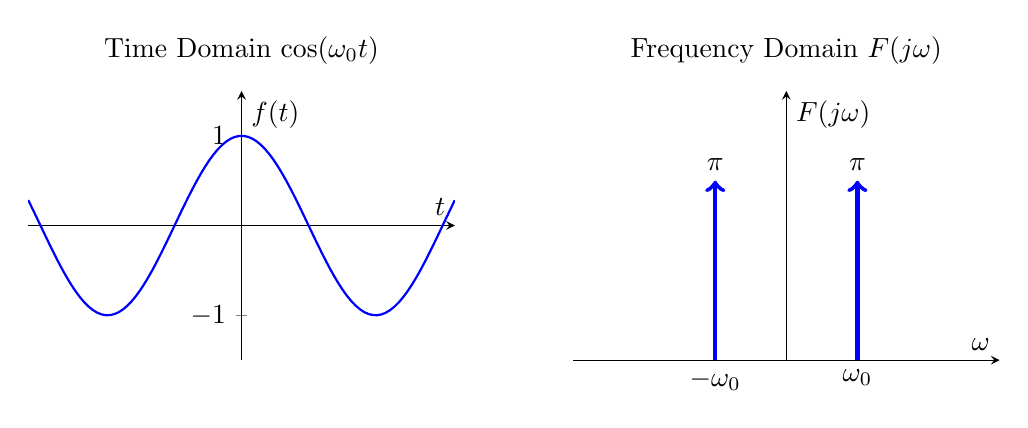
\begin{tikzpicture}
    \begin{groupplot}[
        group style={group size=2 by 1, horizontal sep=1.5cm},
        axis lines = middle,
        width = 7cm, height = 5cm,
        ymin = -1.5, ymax = 1.5,
        ytick = {-1, 1},
        xtick = \empty,
        grid=none,
        xlabel = {$t$},
        ylabel = {$f(t)$}
    ]
        % Time Domain Cosine
        \nextgroupplot[
            title = {Time Domain $\cos(\omega_0 t)$},
            xmin = -5, xmax = 5,
            samples = 100
        ]
        \addplot[thick, blue, domain=-5:5] {cos(deg(x))};

        % Frequency Domain Cosine
        \nextgroupplot[
            title = {Frequency Domain $F(j\omega)$},
            xlabel = {$\omega$},
            ylabel = {$F(j\omega)$},
            xmin = -3, xmax = 3,
            ymin = 0, ymax = 1.5,
            ytick = \empty,
            xtick = \empty,
            clip = false
        ]
        \draw[->, ultra thick, blue] (axis cs:1,0) -- (axis cs:1,1);
        \draw[->, ultra thick, blue] (axis cs:-1,0) -- (axis cs:-1,1);
        \node[anchor=north] at (axis cs:1, 0) {$\omega_0$};
        \node[anchor=north] at (axis cs:-1, 0) {$-\omega_0$};
        \node[anchor=south] at (axis cs:1, 1) {$\pi$};
        \node[anchor=south] at (axis cs:-1, 1) {$\pi$};

    \end{groupplot}
\end{tikzpicture}
\end{document}
